\documentclass[11pt]{article}
\usepackage[letterpaper]{geometry}
\usepackage{MATH562}

\begin{document}
\noindent \textbf{\Large{Caleb Logemann \\
MATH 562 Numerical Analysis II \\
Final Exam
}}

%\lstinputlisting[language=Matlab]{H01_23.m}
\begin{enumerate}
    \item % #1 Done
        Let $A \in \RR^{m \times m}$ be written in the form $A = L + D + U$,
        where $L$ is strictly lower triangular, $D$ is the diagonal of $A$, and $U$
        is the strictly upper triangular part of $A$.
        Assuming $D$ is invertible, $A\v{x} = \v{b}$ is equivalent to
        $\v{x} = -D^{-1}\p{L + U}\v{x} + D^{-1}\v{b}$.
        The Jacobi iteration method for solving $A\v{x} = \v{b}$ is defined by
        \[
            \v{x}^{(n+1)} = -D^{-1}\p{L + U}\v{x}^{(n)} + D^{-1}\v{b}
        \]
        Show that if $A$ is nonsingular and strictly row diagonally dominant:
        \[
            0 < \sum{j \neq i}{}{\abs{a_{ij}}} < \abs{a_{ii}}
        \]
        then the Jacobi iteration converges to $\v{x}_* = A^{-1}\v{b}$ for each
        fixed $\v{b} \in \RR^m$.
        % Hint: the infinity norm is a convenient one to use

        \begin{proof}
            Let $\v{e}_n$ be the error of the nth iteration of the Jacobi iteration
            from the actual solution, that is let
            \[
                \v{e}_n = \v{x}^{(n)} - \v{x}_*.
            \]
            The Jacobi iteration converges to the real solution if
            \[
                \lim{n \to \infty}{\norm[\infty]{\v{e}_n}} = 0 
            \]
            The error vector can be expressed recursively by noting that
            $\v{x}^{(n)}$ is the Jacobi iteration evaluated on $\v{x}^{(n-1)}$
            and that $\v{x}_*$ is a fixed point of the Jacobi iteration as it is
            the true solution to the linear system.
            This means that
            \begin{align*}
                \v{x}^{(n)} &= -D^{-1}\p{L + U}\v{x}^{(n-1)} + D^{-1}\v{b} \\ 
                \v{x}_* &= -D^{-1}\p{L + U}\v{x}_* + D^{-1}\v{b}.
            \end{align*}
            Therefore we can express the error recursively as
            \begin{align*}
                \v{e}_n &= \v{x}^{(n)} - \v{x}_* \\
                \v{e}_n &= \p{-D^{-1}\p{L + U}\v{x}^{(n-1)} + D^{-1}\v{b}} - \p{-D^{-1}\p{L + U}\v{x}_* + D^{-1}\v{b}} \\
                \v{e}_n &= -D^{-1}\p{L + U}\v{x}^{(n-1)} + D^{-1}\p{L + U}\v{x}_* \\
                \v{e}_n &= -D^{-1}\p{L + U}\p{\v{x}^{(n-1)} - \v{x}_*} \\
                \v{e}_n &= -D^{-1}\p{L + U} \v{e}_{n-1}.
                \intertext{Extrapolating this backwards we see that $\v{e}_n$
                    can be expressed in terms of $\v{e}_0$}
                \v{e}_n &= \p{-D^{-1}\p{L + U}}^n \v{e}_{0}.
            \end{align*}
            Now we can consider the limit of $\norm[\infty]{\v{e}_n}$ as $n$
            goes to infinity.
            \begin{align*}
                \lim{n \to \infty}{\norm[\infty]{\v{e}_n}} &= \lim{n \to \infty}{\norm[\infty]{\p{-D^{-1}\p{L + U}}^n \v{e}_{0}}} \\
                \lim{n \to \infty}{\norm[\infty]{\v{e}_n}} &\le \norm[\infty]{\v{e}_{0}} \lim{n \to \infty}{\norm[\infty]{D^{-1}\p{L + U}}^n}
            \end{align*}
            Now consider $\norm[\infty]{D^{-1}\p{L + U}}$.
            The infinity norm is the max row sum of the matrix, that is
            \[
                \norm[\infty]{D^{-1}\p{L + U}} = \max*_{1 \le i \le m} \sum{j=1}{m}{\abs{\p{D^{-1}\p{L + U}}_{ij}}}
            \]
            Because $L + U = A - D$, $\p{L + U}_{ij} = a_{ij}$ if $i \neq j$ and $\p{L + U}_{ii} = 0$.
            Also $D^{-1}$ is diagonal with $\p{D^{-1}}_{ii} = \frac{1}{D_{ii}} = \frac{1}{a_{ii}}$.
            Therefore the matrix product $D^{-1}\p{L + U}$ has entries $\p{D^{-1}\p{L + U}}_{ij} = \frac{a_{ij}}{a_{ii}}$ if $i \neq j$ or 
            if $i = j$, then $\p{D^{-1}\p{L + U}}_{ii} = 0$.
            We can now say that
            \begin{align*}
                \norm[\infty]{D^{-1}\p{L + U}} &= \max*_{1 \le i \le m} \sum{j \neq k}{}{\abs{\frac{a_{ij}}{a_{ii}}}} \\
                \norm[\infty]{D^{-1}\p{L + U}} &= \max*_{1 \le i \le m} \frac{1}{\abs{a_{ii}}} \sum{j \neq k}{}{\abs{a_{ij}}}
                \intertext{However since $A$ is strictly row diagonally dominant $\abs{a_{ii}} > \sum{j \neq k}{}{\abs{a_{ij}}}$,
                    we can conclude that $\frac{1}{\abs{a_{ii}}} \sum{j \neq k}{}{\abs{a_{ij}}} < 1$. Therefore}
                \norm[\infty]{D^{-1}\p{L + U}} &< 1
            \end{align*}
            Since $\norm[\infty]{D^{-1}\p{L + U}} < 1$, it is true that
            $\lim{n \to \infty}{\norm[\infty]{D^{-1}\p{L + U}}^n} = 0$.
            Thus
            \begin{align*}
                \lim{n \to \infty}{\norm[\infty]{\v{e}_n}} &\le \norm[\infty]{\v{e}_{0}} \lim{n \to \infty}{\norm[\infty]{D^{-1}\p{L + U}}^n} \\
                \lim{n \to \infty}{\norm[\infty]{\v{e}_n}} &\le 0
            \end{align*}
            This shows that the error converges to zero, and this proves that
            the Jacobi iteration does converge to the true solution if $A$ is
            strictly row diagonally dominant.
        \end{proof}

    \item % #2
        Let $A \in \RR^{m \times m}$ be symmetric positive definite (SPD),
        $\v{b} \in \RR^m$ and define $\phi:\RR^m \to \RR$ by
        \[
            \phi(\v{x}) = \frac{1}{2}\v{x}^T A \v{x} - \v{x}^T \v{b}
        \]
        Suppose $K$ is a subspace of $\RR^m$.
        Show that $\hat{\v{x}} \in K$ minimizes $\phi(\v{x})$ over $K$ if and
        only if $\nabla \phi(\hat{\v{x}}) \perp K$.

        \begin{proof}
            First let me describe $\nabla \phi(\v{x})$.
            \begin{align*}
                \nabla \phi(\v{x}) &=
                \begin{bmatrix}
                    \frac{\partial \phi}{\partial x_1} \\
                    \cdots \\
                    \frac{\partial \phi}{\partial x_m}
                \end{bmatrix} \\
                \frac{\partial \phi}{\partial x_i} &= \frac{\partial}{\partial x_i} \p{\frac{1}{2} \v{x}^T A \v{x} - \v{x}^T \v{b}} \\
                &= \frac{\partial}{\partial x_i} \p{\frac{1}{2} \sum{j = 1}{m}{x_j \sum{k = 1}{m}{a_{jk} x_k}} - \sum{j = 1}{m}{x_{j} b_j}} \\
                &= \frac{1}{2} \frac{\partial}{\partial x_i} \sum{j = 1}{m}{x_j \sum{k = 1}{m}{a_{jk} x_k}} - b_i \\
                &= \frac{1}{2} \frac{\partial}{\partial x_i} \p{x_i \sum{k = 1}{m}{a_{ik} x_k} + \sum{j \neq i}{}{x_j \sum{k = 1}{m}{a_{jk} x_k}}} - b_i \\
                &= \frac{1}{2} \p{\sum{k \neq i}{}{a_{ik} x_k} + 2a_{ii}x_i + \sum{j \neq i}{}{a_{ji} x_j}} - b_i \\
                &= \frac{1}{2} \p{\sum{k = 1}{m}{a_{ik} x_k} + \sum{j =  1}{m}{a_{ji} x_j}} - b_i \\
                &= \frac{1}{2} \p{\p{A\v{x}}_i + \p{A^T\v{x}}_i} - b_i
                \intertext{This is one entry of the vector $\nabla \phi(\v{x})$ therefore we can write the entire vector as}
                \nabla \phi(\v{x}) &= \frac{1}{2} \p{A\v{x} + A^T \v{x}} - \v{b}
                \intertext{Since $A$ is symmetric, $A = A^T$, this symplifies to}
                \nabla \phi(\v{x}) &= A\v{x} - \v{b}
            \end{align*}

            Now assume that $\nabla \phi(\hat{\v{x}}) \perp K$, therefore
            $\v{x} \cdot \p{A\hat{\v{x}} - \v{b}} = 0$ for any $\v{x} \in K$.
            Let $\v{x} \in K$, then $\v{x} = \hat{\v{x}} + \v{y}$ for some
            $\v{y} \in K$.
            \begin{align*}
                \phi(\v{x}) &= \phi(\hat{\v{x}} + \v{y}) \\
                &= \frac{1}{2}\p{\hat{\v{x}} + \v{y}}^T A \p{\hat{\v{x}} + \v{y}} - \p{\hat{\v{x}} + \v{y}}^T\v{b} \\
                &= \frac{1}{2}\p{\hat{\v{x}}^T + \v{y}^T} A \p{\hat{\v{x}} + \v{y}} - \hat{\v{x}}^T\v{b} - \v{y}^T\v{b} \\
                &= \frac{1}{2}\p{\hat{\v{x}}^TA + \v{y}^TA}\p{\hat{\v{x}} + \v{y}} - \hat{\v{x}}^T\v{b} - \v{y}^T\v{b} \\
                &= \frac{1}{2}\p{\hat{\v{x}}^TA\hat{\v{x}} + \hat{\v{x}}^TA\v{y} + \v{y}^TA\hat{\v{x}} + \v{y}^TA\v{y}} - \hat{\v{x}}^T\v{b} - \v{y}^T\v{b}
                \intertext{Note that $\hat{\v{x}}^TA\v{y} = \v{y}^TA^T\hat{\v{x}} = \v{y}^TA\hat{\v{x}}$ because $A$ is symmetric}
                &= \frac{1}{2}\p{\hat{\v{x}}^TA\hat{\v{x}} + 2\v{y}^TA\hat{\v{x}} + \v{y}^TA\v{y}} - \hat{\v{x}}^T\v{b} - \v{y}^T\v{b} \\
                &= \frac{1}{2}\hat{\v{x}}^TA\hat{\v{x}} - \hat{\v{x}}^T\v{b} + \v{y}^TA\hat{\v{x}} - \v{y}^T\v{b} + \frac{1}{2}\v{y}^TA\v{y} \\
                &= \frac{1}{2}\hat{\v{x}}^TA\hat{\v{x}} - \hat{\v{x}}^T\v{b} + \v{y}^T\p{A\hat{\v{x}} - \v{b}} + \frac{1}{2}\v{y}^TA\v{y} 
                \intertext{We know that $\nabla \phi(\hat{\v{x}}) \perp K$, therefore $\v{y}^T\p{A\hat{\v{x}} - \v{b}} = 0$}
                &= \frac{1}{2}\hat{\v{x}}^TA\hat{\v{x}} - \hat{\v{x}}^T\v{b} + \frac{1}{2}\v{y}^TA\v{y} \\
                &= \phi(\hat{\v{x}}) + \frac{1}{2}\v{y}^TA\v{y}
                \intertext{Since $A$ is positive definite $\v{y}^TA\v{y} \ge 0$ and therefore}
                \phi(\v{x}) \ge \phi(\hat{\v{x}})
            \end{align*}
            This $\hat{\v{x}}$ minimizes $\phi(\v{x})$ over $K$.

            Now assume that $\hat{\v{x}}$ minimizes $\phi(\v{x})$ over $K$.
        \end{proof}

    \item % #3

    \item % #4
        Let $A \in \RR^{n \times n}$ be a symmetric positive definite matrix.
        Let Gaussian elimination be carried out on $A$ without pivoting.
        After $k$ steps, $A$ will be reduced to the form
        \[
            A^{(k)} =
            \begin{pmatrix}
                A_{11}^{(k)} & A_{12}^{(k)} \\
                0            & A_{22}^{(k)} \\
            \end{pmatrix}
        \]
        where $A_{22}^{(k)}$ is an $(n - k) \times (n - k)$ matrix.
        Show by induction
        \begin{enumerate}
            \item[(a)]
                $A_{22}^{(k)}$ is symmetric positive definite.

                \begin{proof}
                    
                \end{proof}

            \item[(b)]
                $a_{ii}^{(k)} \le a_{ii}^{(k-1)}$ for all $k \le i \le n$,
                $k = 1, \cdots, n - 1$.

                \begin{proof}
                    
                \end{proof}
        \end{enumerate}

    \item % #5
        Let $A \in \RR^{m \times n}$ with $m > n$ and
        \[
            A = 
            \begin{pmatrix}
                A_1 \\
                A_2
            \end{pmatrix}
        \]
        where $A_1$ is a nonsingular $n \times n$ matrix, and $A_2$ is an
        $(m - n) \times n$ arbitrary matrix.
        \begin{enumerate}
            \item[(a)] % Done
                What is the pseudo-inverse $A^+$ of $A$ such that $A^+ A = I_n$?
                Express it explicitly in terms of $A_1$ and $A_2$.

                The pseudo-inverse of $A$ is defined as
                \[
                    A^+ = (A^T A)^{-1} A^T
                \]
                Writing this in terms of $A_1$ and $A_2$ results in
                \begin{align*}
                    A^+ &=
                    \p{\begin{pmatrix}
                        A_1^T & A_2^T
                    \end{pmatrix}
                    \begin{pmatrix}
                        A_1 \\
                        A_2
                    \end{pmatrix}}^{-1}
                    \begin{pmatrix}
                        A_1^T & A_2^T
                    \end{pmatrix} \\
                    &= \p{A_1^T A_1 + A_2^T A_2}^{-1}
                    \begin{pmatrix}
                        A_1^T & A_2^T
                    \end{pmatrix}
                \end{align*}

            \item[(b)]
                Prove that $\norm[2]{A^+} \le \norm[2]{A_1^{-1}}$.

                \begin{proof}
                    
                \end{proof}
        \end{enumerate}

    \item % #6 Done
        Let $A \in \CC^{m \times m}$ with $\rank(A) = r$.
        Suppose an SVD of $A$ is given by $A = U\Sigma V^*$, where
        $\v{u}_1, \v{u}_2, \ldots, \v{u}_m$ denote the columns of $U$ and
        $\v{v}_1, \v{v}_2, \ldots, \v{v}_m$ denote the columns of $V$.
        Prove that $\langle\v{v}_{r+1}, \ldots, \v{v}_m\rangle = \null(A)$.

        \begin{proof}
            First let $\v{x} \in \langle\v{v}_{r+1}, \ldots, \v{v}_m\rangle$, then
            $\v{x} = \sum{i = r+1}{m}{b_i \v{v}_i}$.
            If we let $b_i = 0$ for $i = 1, 2, \ldots, r$ and $\v{b} = \br{b_i}$,
            then $\v{x} = V\v{b}$.
            Now consider $A\v{x}$.
            \begin{align*}
                A\v{x} &= U\Sigma V^* V \v{b} \\
                       &= U \Sigma \v{b}
            \end{align*}
            However $\Sigma$ is a diagonal matrix with $\sigma_i$ along the
            diagonal, so $\p{\Sigma \v{b}}_i = \sigma_i b_i$.
            Since $A$ has $\rank(A) = r$, we know that $\sigma_i = 0$ for
            $i \ge r + 1$.
            Therefore if $1 \le i \le r$, then $\sigma_i b_i = 0$ because
            $b_i = 0$.
            If $r + 1 \le i \le m$, then $\sigma_i b_i = 0$ because
            $\sigma_i = 0$.
            Therefore we can conclude that $\Sigma \v{b} = \v{0}$
            Thus $A\v{x} = \v{0}$ and $\v{x} \in \null(A)$.

            Now assume that $\v{x} \in \null(A)$, that is $A\v{x} = \v{0}$.
            \begin{align*}
                A\v{x} &= \v{0} \\
                U\Sigma V* \v{x} &= \v{0} \\
                U^*U\Sigma V* \v{x} &= U^*\v{0} \\
                \Sigma V* \v{x} &= \v{0} \\
                \begin{bmatrix}
                    \sigma_1 \v{v}_1^* \v{x} \\
                    \cdots \\
                    \sigma_r \v{v}_r^* \v{x} \\
                    \sigma_{r+1} \v{v}_{r+1}^* \v{x} \\
                    \cdots \\
                    \sigma_m \v{v}_m^* \v{x}
                \end{bmatrix}
                &= \v{0}
                \intertext{Since $\sigma_i = 0$ for $r + 1 \le i \le m$}
                \begin{bmatrix}
                    \sigma_1 \v{v}_1^* \v{x} \\
                    \cdots \\
                    \sigma_r \v{v}_r^* \v{x} \\
                    0
                    \cdots \\
                    0
                \end{bmatrix}
                &= \v{0}
            \end{align*}
            This implies that $\v{v}_i^* \v{x} = 0$ for $1 \le i \le r$ since
            $\sigma_i > 0$ for $1 \le i \le r$.
            This is equivalent to $\v{x} \perp \v{v}_i$ for $1 \le i \le r$.
            Hence $\v{x} \in \langle \v{v}_1, \cdots, \v{v}_r \rangle^{\perp}$.
            Since $V$ is unitary
            \[
                \langle \v{v}_1, \cdots, \v{v}_r \rangle^{\perp} = \langle\v{v}_{r+1}, \ldots, \v{v}_m\rangle
            \]
            Thus $\v{x} \in \langle\v{v}_{r+1}, \ldots, \v{v}_m\rangle$.
        \end{proof}

    \item % #7
        Problem 33.2 (Page 255) 

    \item % #8
        Problem 36.1 (Page 283)

    \item % #9
        

    \item % #10 Done
        MATLAB project

        Below are the function for performing the 
        Jacobi method, the Gauss-Seidel Method, and the Conjugate Gradient
        method.
        \lstinputlisting[language=Matlab]{Jacobi.m}
        \lstinputlisting[language=Matlab]{GaussSeidel.m}
        \lstinputlisting[language=Matlab]{ConjugateGradient.m}

        The following script uses these three methods to solve the diffusion
        equation $-u_{xx} = 1$ on $x \in \p{0, 1}$.
        It also plots the residual against the number of iterations.
        \lstinputlisting[language=Matlab]{H05.m}
        \begin{center}
            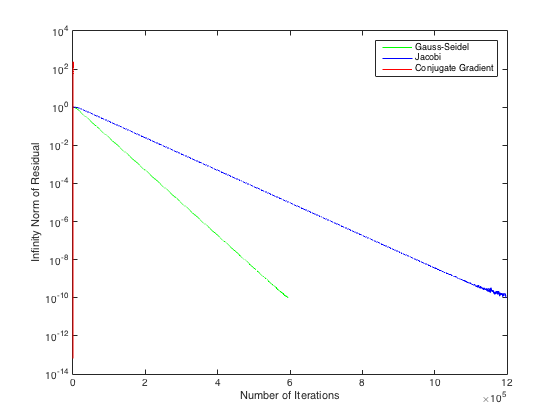
\includegraphics[scale=.7]{Figures/05_10_1.png}
        \end{center}

        We see in this plot that the Gauss-Seidel method converges much faster
        than the Jacobi method.
        Both of these experience linear convergence, but Gauss-Seidel is a faster
        linear convergence.
        The Conjugate Gradient method converges much faster than either of the
        stationary methods.
        The Conjugate Gradient method converges in only 250 steps which is less
        than $m = 500$, the size of the matrix.
\end{enumerate}
\end{document}
